\chapter{User Interface}\label{cha:interface}
This chapter describes the fundamental user interface concepts used by
XCSoar, and is intended as an overview.  More detailed descriptions
are given in following chapters.

\begin{center}
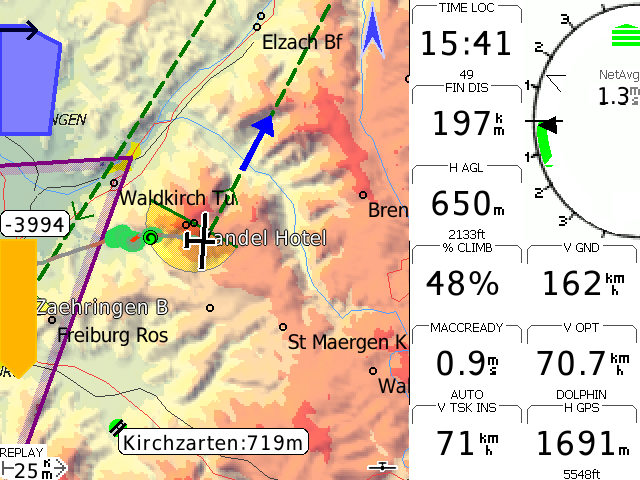
\includegraphics[angle=0,width=\linewidth,keepaspectratio='true']{figures/plain.png}
\end{center}

The XCSoar display is composed of several parts:
\begin{description}
\item[Map area] The bulk of the screen is dedicated to the GPS moving map
display. Various symbols relating to glide computer information are overlaid 
on the map area. Icons and text may appear along the lower edge of the screen
to indicate status of connected devices, operating modes etc.
\item[InfoBoxes] A grid of data values is displayed usually either along
the top and bottom of the screen (portrait display) or to the right of the
screen (landscape display).  These so-called InfoBoxes display data from the
GPS and other input devices as well as data calculated by XCSoar.
\item[Gauges]  Gauges provide instrumentation displays. All gauges are optional
and some may only have meaningful information displayed when XCSoar is
connected to a supported instrument.
\item[Button labels and menus] Hardware buttons on the device running XCSoar
can be used to bring up and navigate smaller on-screen menus that are
typically laid out such that menu items can be selected by pressing the
button adjacent to the item.  If the device has a touch screen, the menu
items can be selected by touching them.  These buttons are drawn in black
text on a grey background.
\item[Status messages] Text is displayed over the map area in status message
boxes.  This text is used to present detailed information to the pilot when
certain events occur.
\item[Dialogue windows] Larger dialogue windows, usually containing graphics and
buttons, are used to present detailed data to the pilot regarding waypoint
details, statistics and analysis etc.
\item[Main menu] The main menu is accessible by double tapping the map area or
InfoBoxes as well as through gesture\gesture{Down - Up}. If the menu buttons are
not pressed after a specified time, they disappear again so as to not obscure the map area.
\end{description}

There are several ways to interact with XCSoar:
\begin{itemize}
\item Touching certain map elements
\item Touching InfoBoxes and on-screen menu buttons
\item `Gesturing', by e.g. drawing a dash from the left to the right
  on the screen (see Section \ref{sec:gestures} below).
\item `Dragging' the screen (touching the screen and moving before releasing).
\item Pressing application buttons on the device.
\item Pressing the cursor keys on the device.
\item Pressing keys or switches on an instrument connected to XCSoar.
\end{itemize}
Depending on the particular hardware used with XCSoar, not all of these methods
of interaction are possible and there may be different numbers or assignments
of buttons.

For the PC version of XCSoar, clicking the mouse over an item is equivalent to
touching it.

Since the Altair does not have a touch screen, all user interaction is performed
via physical buttons, switches or other external interface devices if connected.

\section{The main button menu}
The button menu is a set of buttons drawn on the screen and activated by touch
or hardware button presses.  Using buttons and the button menu is the primary
way the user interacts with XCSoar.

\subsection*{Interface basics}
The menu is organised into four different groups of functions, usually in
the form of a hierarchy.  The specific menu layout depends on the
hardware button configurations and platform, and may also be customised by the
user.

XCSoar can also accept input from external keyboards, game-pads, joysticks,
stick grip switches etc. A wide variety of functions can be assigned to these
inputs.
\sketch{figures/buttonmenu.png}

For Altair, there are four major menus, activated by pressing one of
the vertical strip of hardware buttons on the left of the display.
When a menu is activated, a strip of on-screen buttons appear along the 
bottom of the display.  Pressing the particular menu button again will
cycle through several pages of items.  Pressing the corresponding
horizontal button will activate that item.  At the last page, pressing
the menu button again will turn that menu off and the horizontal strip
of on-screen buttons disappear.  

On the PC version, these mode buttons are activated by the
1, 2, 3 and 4 keys.  The 6, 7, 8, 9 and 0 keys correspond to the horizontal
strip of buttons.

On the PDA version, the mode buttons are activated by the keys to the
side of the joystick/rocker button.

If the user doesn't interact with the computer for some time, the
menu will close automatically.  This menu time-out is configurable.
The escape key on PC, or the PWR/ESC button on Altair, can
also be used to close the current menu.

Menu buttons appear greyed out if the corresponding function is not available. 
For example, the ``Waypoint list'' function will appear grey if there are no waypoints loaded.

Several menu button labels have dynamic text based on context, in
order to make it clearer as to what happens when the button is
pressed.  The convention is used that a button's label describes what
will happen when the button is pressed.  For example, if the button
says \bmenu{MC Auto}, then pressing the button will turn on `Auto
MacCready', and the button label will then change to \bmenu{MC Manual}. 
In the menu list described below, generic labels are used.

\subsection*{Menu function groups}
This section describes the default layout of the menu system on all
platforms.  The functions performed by each button are explained more
fully in following chapters.

The primary menu buttons are activated by each of the vertical strip of buttons
on Altair, from top to bottom:
\begin{jspecs}
\item[\bmenu{Nav}] Actions for navigation control, primarily cross-country
gliding tasks.
\item[\bmenu{Display}] Actions to control the display.
\item[\bmenu{Config}] Configuration of XCSoar, connected devices, and in-flight
settings.
\item[\bmenu{Info}] Activates various informational dialogue windows.
\end{jspecs}

For the PC version, the keys 1, 2, 3 and 4 activate the 
corresponding menu.  The following menu item list has on the left side of most 
of the menu buttons links to the respective section. Follow them to get to all 
related details.

\section{Menu item overview}

\subsection*{Navigation menu}
\noindent\makebox[\textwidth]{%
\begin{tabularx}{1.8\textwidth}{l|ccccc}

Nav 1/2 & \ref{cha:tasks}\bmenus{Task}
 & {\bmenut{Previous}{Turnpoint}} & {\bmenut{Next}{Turnpoint}}
 & \ref{sec:waypoint-selector-dialog}\bmenut{Waypoint}{List}
 & \ref{sec:alternates}\bmenus{Alternates} \\ \\
Nav 2/2 & \ref{sec:taskabort}\bmenut{Task}{Abort}
 & \ref{sec:markers}\bmenut{Mark}{Drop}
 & {}
 & \bmenus{Target}
 & \ref{sec:waypointdetails}\bmenut{Waypoint}{Details}

\end{tabularx}}

You should not start using XCSoar without knowing about the `Alternates' feature. 
Any `Task' related item in the navigation menu are used for planned cross 
country flight and certainly the second step.

\subsection*{Display menu}
\noindent\makebox[\textwidth]{%
\begin{tabularx}{1.9\textwidth}{l|ccccc}

Display 1/2 & \ref{sec:zooming}\bmenut{Zoom}{In}
 & \bmenut{Zoom}{Out} & \bmenut{Zoom}{Auto}
 & \bmenus{Info Cruise}
 & \ref{sec:panning}\bmenut{Pan}{On} \\ \\
Display 2/2 &  \ref{sec:maplabels}\bmenut{Labels}{All/...}
 & \ref{sec:trail}\bmenut{Trail}{Full/...}
 & \bmenut{Terrain}{On/Off}
 & \ref{sec:terrain_topo}\bmenut{Topo.}{On/Off}
 

\end{tabularx}}

Most of the display menu items are available on gestures, or special key 
short-cuts of your device. Once you are familiar with XCSoar you probably 
will use those menu items less frequently.

\subsection*{Configuration menu}
\noindent\makebox[\textwidth]{%
\begin{tabularx}{1.9\textwidth}{l|ccccc}

Config 1/3 & \bmenut{MacCready}{$+$} & \ref{sec:stf}\bmenut{MacCready}{$-$}
 & \ref{sec:auto-maccready}\bmenut{MacCready}{Auto}
 & \ref{sec:flight-setup}\bmenut{Flight}{Setup}
 & \ref{sec:wind-setup}\bmenut{Setup}{Wind} \\ \\
Config 2/3 & \bmenus{Vega}
 & \ref{cha:configuration}\bmenut{Setup}{System}
 & \ref{sec:airspace-filter}\bmenut{Settings}{Airspace}
 & \ref{sec:logger}\bmenut{Logger}{Start}
 & \ref{sec:logger-replay}\bmenus{Replay} \\ \\
Config 3/3 & \ref{sec:raw-logger}\bmenus{Raw Logger}
 & \ref{conf:comdevices}\bmenus{Devices}
 & \bmenus{Setup Plane}
 & \bmenut{File}{Manager}

\end{tabularx}}

The configuration menu is typically part of the ground interaction with 
XCSoar. You are not expected to spend much time in-flight with tweaking 
the configuration, except you manually adjust wind or MacCready settings. 
The `Vega' item gives control over the  Vega intelligent variometer. This 
comprises a sub-menu.


\subsection*{Information menu}
\noindent\makebox[\textwidth]{%
\begin{tabularx}{1.8\textwidth}{l|ccccc}

Info 1/3 & \ref{sec:flarm-traffic}\bmenut{FLARM}{Radar}
 & \bmenut{METAR}{TAF} & \bmenut{What's}{here?}
 & \ref{sec:checklist}\bmenut{Check}{list}
 & \ref{sec:analysis-climb}\bmenus{Analysis} \\ \\
Info 2/3 & \ref{sec:flight-status}\bmenus{Status}
 & \ref{sec:weather-forecast}\bmenus{Weather}
 & \ref{sec:team-flying}\bmenut{Team}{Code}
 & \bmenut{FLARM}{Details}
 & \ref{sec:team-flying}\bmenut{Thermal}{Assistant} \\ \\
Info 3/3 & \ref{sec:credits}\bmenus{Credits}
 & \bmenut{Message}{Repeat}

\end{tabularx}}

The information menu is always a good address, when not only a clue on 
how to set MacCready is requested, but rather more elaborate help on a 
larger scope tactical decision on your flight is requested.


\subsection*{The Vega variometer sub-menu of the configuration menu}

\noindent\makebox[\textwidth]{%
\begin{tabularx}{1.8\textwidth}{l|ccccc}

Vega 1/2 & \bmenut{Airframe}{Switches} & \bmenut{Setup}{Audio}
 & \bmenut{Manual}{Demo} & \bmenut{Setup}{Stall} & \bmenus{Accel} \\ \\
Vega 2/2 & \bmenut{ASI}{Zero} & \bmenut{Accel}{Zero}
 & \bmenus{Store} & \bmenut{Cruise}{Demo} & \bmenut{Climb}{Demo}

\end{tabularx}}

The functions in this sub-menu require the Vega intelligent variometer. 
The menu can only be accessed if `Vega' is selected as the connected device.

\subsection*{The pan mode sub-menu of the Display menu}

\noindent\makebox[\textwidth]{%
\begin{tabularx}{1.6\textwidth}{l|ccccc}
Pan & \bmenut{Pan}{Off} & \ref{sec:panning}\bmenut{Zoom}{in} & \bmenut{Zoom}{out}
 & \bmenut{What's}{here?}
\end{tabularx}}

This sub-menu unfortunately overlays the full-screen map view of the pan mode.
 It's functions are quite evident, although the menu could be replaced by multi-touch
 technology or knobs (like on Altair). Besides the essential `exit pan mode'
 function the `What's here?' button offers brilliant access to the variety of
 information of the map.

\section{Default menu buttons}

When no menu is active, (so-called default mode), the horizontal row
of buttons in Altair perform the following functions (from left to right):

\begin{center}
\begin{tabular}{c c c c c c}
 PC: & 6 & 7 & 8 & 9 & 0 \\
 Altair: & F5 & F6 & F7 & F8 & F9 \\
& \bmenut{Flight}{Setup} & \bmenut{Task}{Manager} & {} &
\bmenus{Target} & \bmenut{Drop}{Mark} \\
\end{tabular}	
\end{center}

Pressing ESC on Altair displays labels for these default menu buttons.

For all other versions in the default mode, the cursor keys perform
the following functions:
\begin{jspecs}
\item[Up key] Zoom in
\item[Down key] Zoom out
\item[Left key] Drop marker
\item[Right key] Toggle through normal/aux. InfoBoxes and full-screen
\item[Enter] Clear status message or suppress FLARM gauge if open and no warning
active
\end{jspecs}

For the Altair version in the default mode, the rotary knob performs
the following functions:
\begin{jspecs}
\item[Outer knob counter-clockwise] Zoom in
\item[Outer knob clockwise] Zoom out
\item[Inner knob counter-clockwise] (No function assigned)
\item[Outer knob clockwise] (No function assigned)
\item[Knob button press] Clear status message or acknowledge airspace warning
\end{jspecs}

In dialogue forms, the rotary knob in Altair performs the role of the cursor and
enter keys:
\begin{jspecs}
\item[Outer knob counter-clockwise] Up cursor
\item[Outer knob clockwise] Down cursor
\item[Inner knob counter-clockwise] Left cursor
\item[Inner knob clockwise] Right cursor
\item[Knob button press] Enter key
\end{jspecs}

For Altair, the buttons along the edge of the display can be used as
alternate ways of navigating in dialogues.  The F4 key (directly above
the rotary knob) can be used as an alternate ENTER key (instead of
pressing the rotary knob) in dialogues.  The F6 and F7 keys (directly to
the right of the rotary knob) can be used to select the next or
previous page in multi-page dialogues.

\subsection*{Dynamic menu labels}
Certain menu items have dynamic labels to make it clearer what happens when the
menu item is selected.  Furthermore, items that are not available are greyed
out to indicate that selecting the menu item will not do anything.

The convention used for dynamic menu labels is for the labels to display the
action that will be performed once the menu item is selected. For example 
``Lights On'' will turn the lights on, and the menu will be updated to display
``Lights Off'', which would then if pressed turn the lights off. This
convention is used throughout XCSoar.

A selection of key dynamic menu items is presented below:
\begin{description}
\item[\bmenu{Next turnpoint}]  
  Greyed out if the task is cleared, or if the active turnpoint is the
  finish. If the currently active turnpoint is the turnpoint prior to the 
  finish, this displays  ``Waypoint finish''.
\item[\bmenu{Previous turnpoint}]  
  Greyed out if the task is cleared, or if the active turnpoint is the
  start and there are no multiple start points.  If there are multiple
  start points and the active turnpoint is the start, then this
  displays ``Cycle start'' to allow selection between the various
  start points.  If the active turnpoint is the first turnpoint after 
  the start, this displays ``Waypoint Start''.
\item[\bmenu{Labels}]  
  This now displays ``Labels On'', ``Labels MID'' or ``Labels Off''.
\item[\bmenu{Task calculator}]  
  Greyed out if the task is cleared or in task abort.
\item[\bmenu{Arm Advance}]  
  Greyed out if Auto or Manual advance mode is active.  Displays ``Arm
  start'' when the active turnpoint is the start and the trigger is
  not armed.  Displays ``Arm Cancel'' if the trigger is armed.
  Displays ``Arm turn'' if the active turnpoint is past the start.
\item[\bmenu{Task Edit}]
  Greyed out if there is no waypoint database.
\end{description}

\section{InfoBoxes and screen pages}

The information displayed in the InfoBox fields can be selected from a
wide variety of options (listed in Chapter~\ref{cha:infobox}). These
fields can also be used to change for example the MacCready setting.

The specific number and layout of the InfoBox grid depends on the
screen orientation and the device's display size.  

For a 320x240 display
Pocket PC in portrait mode, there are four InfoBoxes above and four
InfoBoxes below the map display.  
\sketch{figures/infoboxes.png}

A typical landscape layout has 9 InfoBoxes and the variometer gauge 
to the right of the map display. 
 
For larger displays are up to 24 InfoBoxes on one screen page possible.

\subsection*{Pages with different InfoBox sets}

XCSoar allows the pilot to define various sets of InfoBoxes that are 
appropriate to various stages of flight (e.g. when circling in a thermal, 
flying between thermals, on final glide, etc.). XCSoar can be configured 
to automatically switch from one screen page to another based on the mode 
of flight, or you can manually roll through the various pages, including 
one with a full-screen map and no InfoBoxes at all. Thus a screen page 
consists of a InfoBox set and specific map appearance, that includes 
map orientation and scale.

To toggle through the various InfoBox pages, using the left/right cursor 
keys (Altair), or by gestures (touch-screen).
\gesture{Right or Left} 


\subsection*{Modifying InfoBox values}
(This section applies only when a touch-screen or mouse is present.)

Some InfoBox values can be changed by the user by selecting (i.e. long-pressing) the
InfoBox with the touch-screen or mouse.  This brings up a small tabular dialogue:

\begin{description}
\item[\bmenu{Edit}]  
  Allows the pilot to adjust the InfoBox setting (e.g. raise or lower the 
  MacCready setting)

\item[\bmenu{Setup}]
  Allows you to change the behaviour of the setting related to the InfoBox 
  (for example, changing from Auto to Manual MacCready setting mode); or 
  to change the InfoBox itself by pressing \bmenu{Switch InfoBox}, then 
  choosing from a list of all available InfoBoxes.

\end{description}


Examples of InfoBoxes that can
be adjusted include MacCready setting, wind speed, and height (QNH).

\subsection*{Changing InfoBox sets}
An InfoBox set can either be composed by calling the configuration dialogue 
from the menu: \begin{center}
\bmenu{Config 2}\blink\bmenu{Setup System}
\end{center}
on the `Look / InfoBox Modes' setup page or by
performing a long press on the InfoBox that should be changed. In the second 
case a list dialogue opens, giving you all available InfoBoxes to choose from.

\section{Status messages}
Status messages appear over the map area to present text for a short period of
time.  The message disappears after the time period has elapsed, and different
types of message have different periods. Additionally, status messages can be
made to disappear by acknowledging the message.  Acknowledgement is achieved by
either pressing the enter key (rotary knob on Altair), touching the status
message (on touch-screen devices) or clicking the screen (mouse enabled devices).

Additional user buttons may be assigned to a status message repeat function,
which brings up the last message again.

Typical status messages include:
\begin{itemize}
\item Airspace queries
\item Airspace warnings
\item User interface events (e.g.\ changing display modes)
\item Glide computer events (e.g.\ take-off, turning waypoints)
\end{itemize}

Note that status messages do not appear while a dialogue is on screen, the
messages are buffered and displayed as soon as the dialogue is exited.

\section{Dialogue windows}\label{sec:dialog-windows}

XCSoar contains several dialogue windows that can be activated to bring up
additional information and are also used for more complex interactions with the
user, such as editing tasks and configuring settings.

Some dialogues simply display information, and require no user input. Other
dialogues contain data fields that can be modified or buttons that can be pressed.  

A cursor appears over the active button or data field. Pressing the up/down
arrow keys (or rotating the outer knob on Altair), the cursor will cycle
through the next or previous items. For list items and scrollable text, the
up/down arrow key moves the cursor up or down the list or text, and the
left/right arrow keys move the cursor up or down by one page in long lists.

For PDAs and PC versions, list items can be selected by touching the item (or
left-clicking with the mouse). Once a list item is selected, another touch
(left click) is equivalent to pressing the enter key.

Pressing the right/left arrow keys (or rotating the inner knob on Altair), the
data field value under the cursor can be modified. Pressing the enter key (or
pressing the rotary knob on Altair) activates the button or makes a selection
from a list.

Dialogues are typically started from the button menu.  

Many of the dialogue windows have multiple pages of information and are controlled
in a consistent fashion. Press the \button{$<$} or \button{$>$} buttons to
select the next or previous page of the dialogue and the \button{Close} button to
make the dialogue disappear.

The escape key on a PC or the PWR/ESC button on Altair, can also be used to
close dialogues.

The user must close the dialogue to return to the normal map mode. When a dialogue
has been opened, the main button menu is disabled until the dialogue is closed.

In some dialogues, items that are not relevant or valid (such as AAT details when
flying a non-AAT task) are not displayed.

A summary of the major dialogues is presented below.
\begin{description}
\item[Flight setup] Used to modify the polar of the glider both before and
during flight, as well as to set the QNH pressure
\item[Wind] Used to modify or adjust the estimated wind magnitude and direction
\item[Waypoint details] Describes a waypoint in detail and has navigation
functions such as `GoTo' and `Insert in Task'
\item[Waypoint list] Used to select a waypoint from the waypoint database
\item[Task manager] Used to create, modify and view cross country tasks
\item[Analysis] Shows several pages of analysis and statistics about the flight
\item[Status] The status dialogues give summaries of the situation of the 
aircraft, system, task, start and times
\item[Configuration] Allows XCSoar and certain connected devices to be
configured
\item[Airspace filter] Controls enabling and disabling the display and warnings
of each airspace class
\item[Team code] Allows transfer of coordinates between FLARM team mates via a 
  code
\item[Devices]  Selection of various external devices (e.g. smart variometers, 
  FLARM, etc.).
\item[Setup Plane]  Easy reconfiguration of the plane-dependant settings (e.g. 
  polar, competition ID, etc.) by choosing from a list of previously-created 
  plane profiles.
\end{description}

These dialogues are described in later chapters. with the exception of the
check-list, status and text entry dialogues, which are described below.

\subsection*{Check-list (dialogue example)}\label{sec:checklist}
The checklist dialogue can display several pages of user-defined free text.
Typically this is used for check-lists. It can be accessed via the menu under 
\begin{quote}
\bmenu{Info 1}\blink\bmenu{Check list}
\end{quote}

These check-lists may include: daily inspection, preflight, out-landing,
pre-landing, radio procedures, and aircraft rigging and de-rigging
instructions.  Since the check-lists may be long, the up/down keys (or rotary
knob on Altair) may be used to scroll through the text. Clicking the
\button{$<$} and \button{$>$} buttons selects the previous/next checklist.

\begin{center}
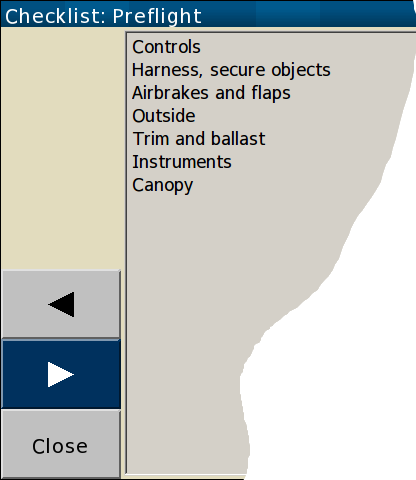
\includegraphics[angle=0,width=0.8\linewidth,keepaspectratio='true']{figures/checklist.png}
\end{center}


\subsection*{Text entry} \label{sec:textentry}
A text entry dialogue is used for entering text.  This is used for team
code entry, setting file names, waypoint editing, as well as entering
other configuration options, such as pilot name for the logger.

Two ways of entering text are provided. See Section~\ref{sec:status} for 
details on customisation.

To enter text in `high score style', use the A+/A- buttons to adjust the 
character under the cursor (underlined character). Clicking the \button{$<$} 
and \button{$>$} buttons move the cursor left/right.  

\begin{center}
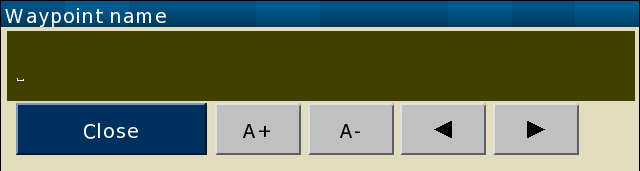
\includegraphics[angle=0,width=0.6\linewidth,keepaspectratio='true']{figures/textentry.png}
\end{center}

To enter text with the touch screen keyboard, press the letters of choice 
one after the other. In some dialogues (e.g. waypoint editing) only the next 
letters matching to an entry in the database will be shown. For deleting the 
last letter use the \button{$<-$} button. The \button{Clear} button deletes all input.

\begin{center}
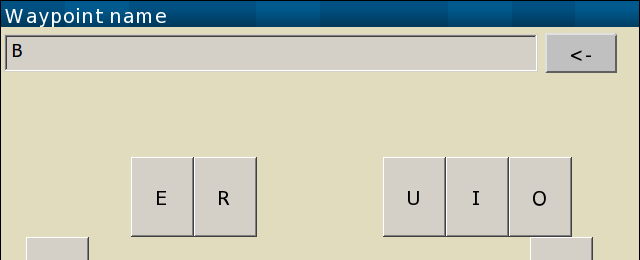
\includegraphics[angle=0,width=0.6\linewidth,keepaspectratio='true']{figures/textentry_keyboard.png}
\end{center}

Press \button{Ok} to take over, or \button{Cancel} to exit.

\section{Acoustic alert and sound feedback}

XCSoar generates sounds for different events, and can be configured to
have custom sounds for any event.  See Section~\ref{sec:status} for
details on customisation.

When XCSoar is connected to the Vega intelligent variometer, it sends
commands to Vega's speech system, to give verbal cues and warnings such as:
\begin{itemize}
\item Final glide through terrain
\item Approaching/passing a task waypoint
\item Airspace warnings
\end{itemize}

The XCSoar user interface also can connect sound feedback to the completion 
of any command like:
\begin{itemize}
\item Marker dropped
\end{itemize}

\section{Screen visuals}

Certain aspects of the look of items on the screen can be adjusted.
The most noticeable of these is whether to display InfoBoxes and
gauges in black on white (called inverse colours) or white on black.

For Altair the control of the screen hardware 
brightness can be controlled from the brightness dialogue
accessible from the menu:
\begin{quote}
\bmenu{Display 2}\blink\bmenu{Bright}
\end{quote}
\sketch{figures/brightness.png}

Refer to the {\em Altair User's Manual} for details of the brightness
dialogue.


\section{Help system}
A help system now provides descriptive text for properties in
most dialogues.  When a property is selected, for Altair, press and hold the
enter button for two seconds, then release.  A window will open with
help text describing the property.

\section{Interfacing with gestures}\label{sec:gestures}
As of version 6.0, XCSoar supports so-called `gestures'.

To use this feature hold down the finger on the 
touch-screen (or mouse button at the PC), draw a certain figure and release 
the touch-screen / mouse button. Depending on the figure that was drawn 
a certain function is activated. A list of generally available gestures is 
shown below. 

A figure is defined by movements of the 
cursor in the four directions Up, Down, Left and Right. This means if 
you drag your finger down and afterwards to the right over the screen, 
\gesture{down-right} the gesture "DR" is detected, which stands for "Down-Right". 
It will bring up the waypoint list. The manual indicates an available 
gesture as shown here on the left side of the text body.

Generally available gestures on the map screen:
\begin{itemize}
\item U: Zoom in
\item D: Zoom out
\item L: Toggle map mode pro-grade (Normal, Aux. InfoBoxes, Full-screen)
\item R: Toggle map mode retrograde (Full-screen, InfoBoxes, Aux., Normal)
\item DU: Show the menu
\item DR: Show the Select Waypoint dialogue
\item RD: "T" opens the task dialogue
\end{itemize}

